\section{Método}

\subsection{Datos}
Para entrenar nuestras redes neuronales artificiales y probar los ataques adversarios y las defensas contra ellos, se emplearon las dos bases de datos más sencillas para procesamiento de imágenes: MNIST y CIFAR-10.

\subsubsection{MNIST}
La base de datos MNIST es un compendio de los dígitos del 0 al 9 en letra manuscrita con 60,000 imágenes para entrenar a distintos sistemas de procesamiento de imágenes y 10,000 imágenes para evaluarlos. Se trata de un subconjunto de imágenes de un conjunto más grande que compiló el National Institute of Standards and Technology (NIST) del Departamento de Comercio los EEUU. Las siglas MNIST database significan Modified NIST database. Es una buena base de datos para probar técnicas de aprendizaje y métodos de reconocimiento de patrones con datos del mundo real empleando un esfuerzo mínimo en preprocesamiento y formato. En la Figura \ref{mnist_train} se muestran 100 imágenes del conjunto de entrenamiento y en la Figura \ref{mnist_test} se muestran 100 imágenes del conjunto de evaluación.

\begin{figure}[h!]
    \centering
    \begin{subfigure}[b]{0.47\textwidth}
        \centering
        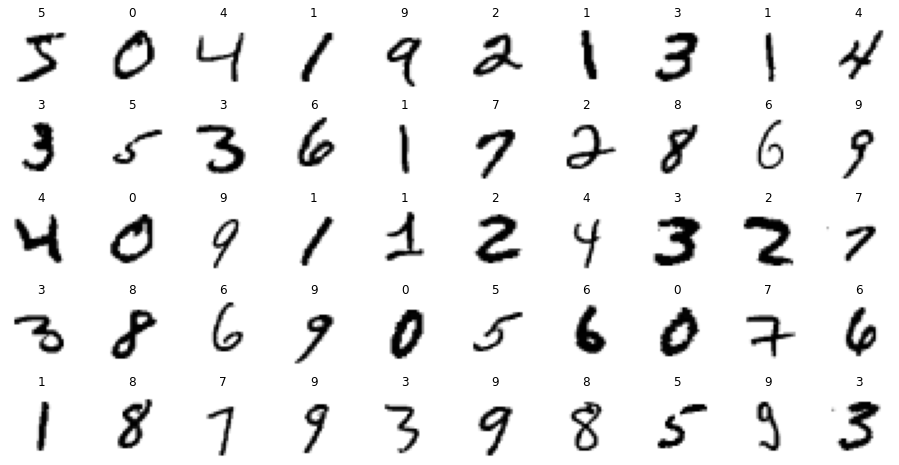
\includegraphics[width=\textwidth]{images/mnist/mnist_train_first50.png}
        \caption{Primeras 50 imágenes del conjunto \texttt{train} de MNIST con sus respectivas etiquetas.}
        \label{mnist1}
    \end{subfigure}
    \hspace{1em}
    \begin{subfigure}[b]{0.47\textwidth}
        \centering
        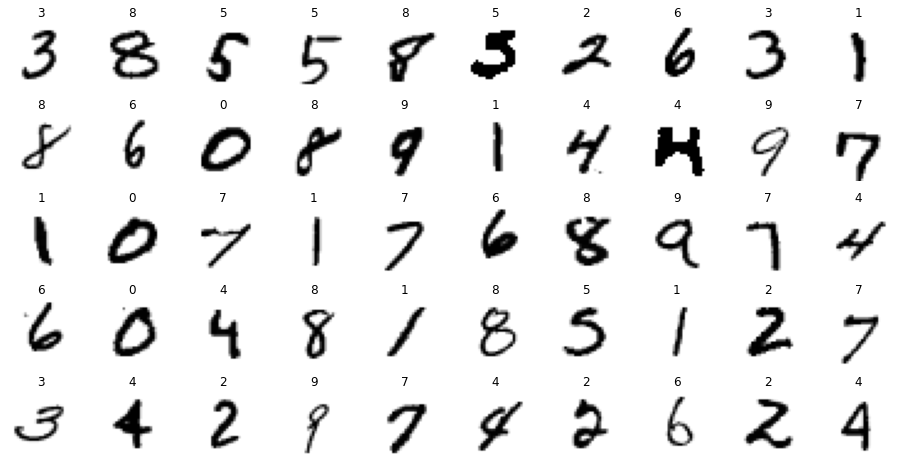
\includegraphics[width=\textwidth]{images/mnist/mnist_train_random.png}
        \caption{50 imágenes aleatorias del conjunto \texttt{train} de MNIST con sus respectivas etiquetas.}
        \label{mnist2}
    \end{subfigure}
    \caption{Imágenes del conjunto de entrenamiento (train) de MNIST}
    \label{mnist_train}
\end{figure}

\begin{figure}[h!]
    \centering
    \begin{subfigure}[b]{0.47\textwidth}
        \centering
        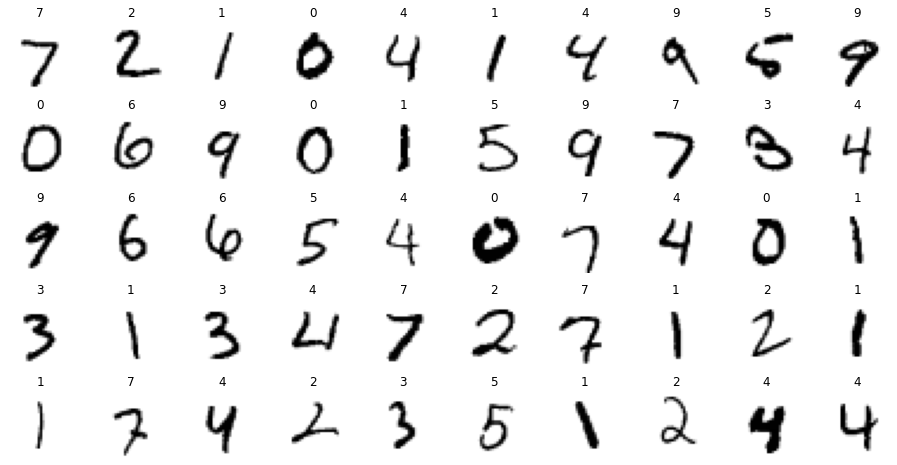
\includegraphics[width=\textwidth]{images/mnist/mnist_test_first50.png}
        \caption{Primeras 50 imágenes del conjunto \texttt{test} de MNIST con sus respectivas etiquetas.}
        \label{mnist3}
    \end{subfigure}
    \hspace{1em}
    \begin{subfigure}[b]{0.47\textwidth}
        \centering
        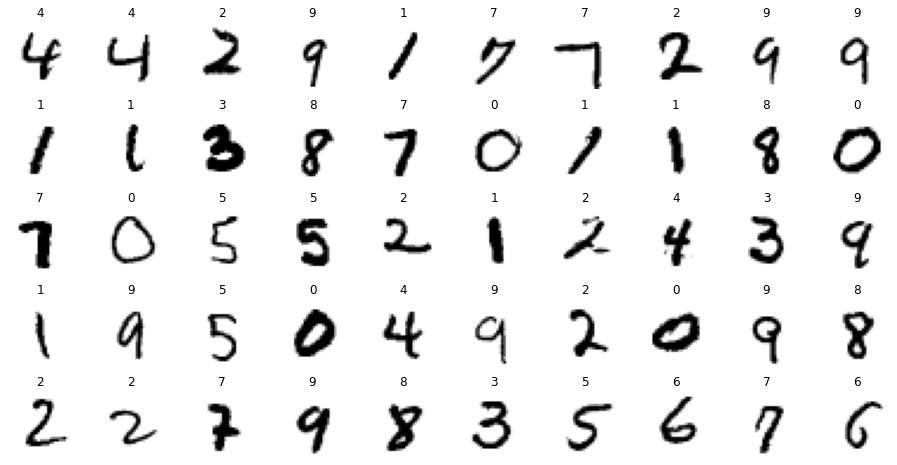
\includegraphics[width=\textwidth]{images/mnist/mnist_test_random.png}
        \caption{50 imágenes aleatorias del conjunto \texttt{test} de MNIST con sus respectivas etiquetas.}
        \label{mnist4}
    \end{subfigure}
    \caption{Imágenes del conjunto de evaluación (test) de MNIST}
    \label{mnist_test}
\end{figure}

De las 10,000 imágenes de evaluación, la mitad fueron escritas por estudiantes de preparatoria y la otra mitad por empleados de la oficina de censos, mientras que de las 60,000 imágenes de entrenamiento, 58,527 de los números fueron escritos por 500 estudiantes y el resto por los empleados. El tamaño de estas imágenes en blanco y negro fue normalizado a una caja de 20$\times$20 pixeles y se colocó su centro de masa en un campo de 28$\times$28 \cite{lecun2010mnist}. Cabe recalcar que la distribución de los dígitos en MNIST no es homogénea, como puede observarse en la Figura \ref{mnist_dist}.

\begin{figure}[h!]
    \centering
    \begin{subfigure}[b]{0.45\textwidth}
        \centering
        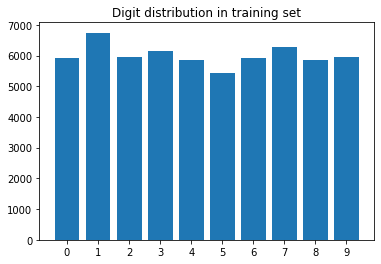
\includegraphics[width=\textwidth]{images/mnist/dist_train.png}
        \caption{Distribución de los dígitos en el conjunto de entrenamiento de MNIST}
        \label{mnist7}
    \end{subfigure}
    \hspace{1cm}
    \begin{subfigure}[b]{0.45\textwidth}
        \centering
        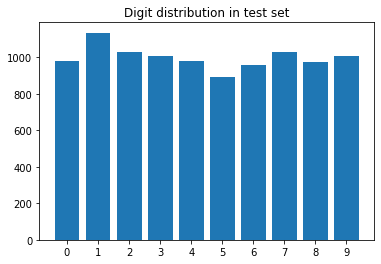
\includegraphics[width=\textwidth]{images/mnist/dist_test.png}
        \caption{Distribución de los dígitos en el conjunto de evaluación de MNIST}
        \label{mnist8}
    \end{subfigure}
    \caption{Distribución de los dígitos en MNIST}
    \label{mnist_dist}
\end{figure}

\subsubsection{CIFAR-10}
Los grupos del MIT y la NYU recopilaron un conjunto de millones de diminutas imágenes en color de la web, se trata de un excelente conjunto de datos para el entrenamiento no supervisado de modelos generativos profundos. Se crearon dos juegos de etiquetas confiables: el conjunto CIFAR-10, que tiene 6000 ejemplos de cada una de 10 clases y el conjunto CIFAR-100, que tiene 600 ejemplos de cada una de 100 clases que no se superponen. Usando estas etiquetas, se mostró que el reconocimiento de objetos mejora significativamente al entrenar previamente una capa de características en un gran conjunto de imágenes diminutas sin etiquetar.

Esta base de datos fue ensamblada buscando en la web imágenes de cada sustantivo en inglés no abstracto en la base de datos léxica WordNet. Utilizaron varios motores de búsqueda, incluidos Google, Flickr y Altavista y mantuvieron aproximadamente los primeros 3000 resultados para cada término de búsqueda. Después de recopilar todas las imágenes para un término de búsqueda en particular, eliminaron duplicados perfectos e imágenes en las que una parte excesivamente grande de los píxeles eran blancos, ya que tendían a ser figuras sintéticas en lugar de imágenes naturales. El término de búsqueda utilizado para encontrar una imagen le proporciona una etiqueta aproximada, aunque es extremadamente poco confiable debido a la naturaleza de la tecnología de búsqueda de imágenes en línea. En total, el conjunto de datos contiene 80 millones de imágenes en color reducidas a 32×32 y distribuidas en 79,000 términos de búsqueda \cite{Krizhevsky09learningmultiple}.

\begin{figure}[h!]
    \centering
    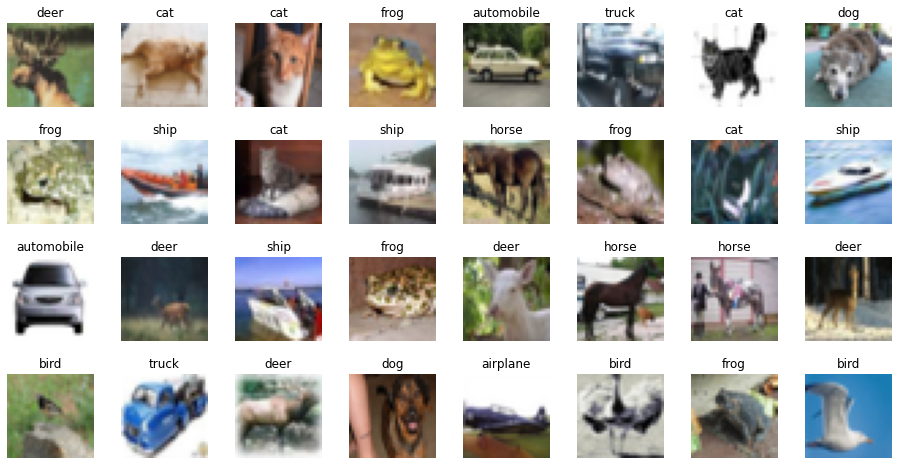
\includegraphics[width=\textwidth]{images/cifar-10/cifar10.png}
    \caption{Algunas imágenes de la base de datos CIFAR-10}
    \label{cifar}
\end{figure}

El conjunto de datos se divide en cinco lotes de entrenamiento y un lote de prueba, cada uno con 10,000 imágenes. El lote de prueba contiene exactamente 1000 imágenes seleccionadas al azar de cada clase. Los lotes de entrenamiento contienen las imágenes restantes en orden aleatorio, pero algunos lotes de entrenamiento pueden contener más imágenes de una clase que de otra. Entre ellos, los lotes de entrenamiento contienen exactamente 5000 imágenes de cada clase \cite{cifarsite}. 

Las 10 clases de CIFAR-10 se encuentran en orden alfabético y son:
\begin{multicols}{5}
\begin{enumerate}
    \item airplane
    \item automobile
    \item bird
    \item cat
    \item deer
    \item dog
    \item frog
    \item horse
    \item ship
    \item truck
\end{enumerate}
\end{multicols}


\subsection{Ataques}

\subsubsection{Fast Gradient Method}
\cite{goodfellow2015explaining}, maybe more

Sean $\theta$ los parámetros de un modelo, $x$ la entrada, $y$ las salidas asociadas, y $J(\theta, x, y)$ la función de costo. La función de costo se linealiza alrededor del valor actual de $\theta$. Sea $\epsilon \in \mathbb{R}^+$. Definamos la imagen adversaria 
\[\tilde{x} = x + \epsilon \eta_{\text{opt}}\]
Se puede definir $\eta_{\text{opt}}$ por el problema de optimización
\[\eta_{\text{opt}} = \operatornamewithlimits{argmax}_{\eta}\left\{ \operatorname{grad} ^\top \eta: \norm{\eta}_p< \epsilon\right\}\]
Donde $p \in \mathbb{N} \cup \{\infty\}$ y $\operatorname{grad} = \nabla_x J(\theta, x, y)$. Experimentamos con dos valores de $p$:
\begin{enumerate}[a)]
    \item $p = 2$,
    \[\eta_{\text{opt}} = \frac{\operatorname{grad}}{\norm{\operatorname{grad}}}\]
    \item $p = \infty$,
    \[\eta_{\text{opt}} = \operatorname{sign}(\nabla_x J(\theta, x, y))\]
\end{enumerate}


\subsubsection{Carlini \& Wagner}
Nicholas Carlini y David Wagner \cite{carlini2017evaluating} propusieron en 2017 un método para encontrar ejemplos adversarios que tuvieran poca distorsión en la norma $L^2$. Dada $x$, se escoge una clase $t$ y se busca la $\omega$ que resuelva
\begin{equation*}
    \text{minimize} \quad \Big\lVert \dfrac{1}{2}\big(\tanh(\omega) + 1\big) - x \Big\rVert^2 + c\cdot f\bigg(\dfrac{1}{2}\big(\tanh(\omega) + 1\big)\bigg)
\end{equation*}
con $f$ definida como
\begin{equation*}
    f(x') = \text{max}(\ \text{max}\{Z(x')_i : i\neq t\} - Z(x')_t\ ,\ -\kappa\ )
\end{equation*}
Esta $f$ está basada en una función objetivo en la que se controla la confianza con la que ocurre una clasificación errónea al ajustar el valor de $\kappa$. El parámetro $\kappa$ sugiere a quien esté resolviendo el problema encontrar una instancia adversaria $x'$ que sea clasificada con mucha confianza como la clase $t$. Ellos toman $\kappa = 0$. $Z(x)$ es el logit para $x$, es decir la pre-activación de la capa de salida softmax.

En la Figura \ref{CW} se observa que el ataque es totalmente imperceptible para nosotros. Aunque este ataque puede ser dirigido, se usa de la forma no dirigida en este reporte: en la Figura \ref{attack_examples} se muestra el tipo de ruido que generan los ataques FGSM, FGM y Carlini-Wagner, los cuales son cada vez más sutiles en ese respectivo orden, y con esos tres ataques se logra que la red clasifique erróneamente un 8 por un 3.

\begin{figure}[h!]
    \centering
    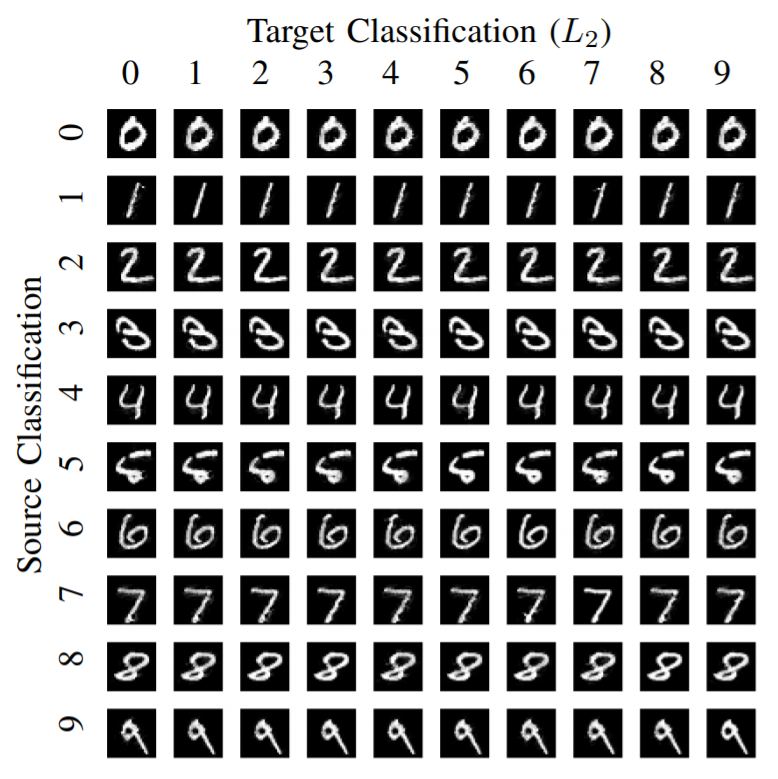
\includegraphics[width=0.5\textwidth]{images/CW/CW_L2.png}
    \caption{Ataque de Carlini \& Wagner con la norma $L^2$ sobre MNIST aplicando un ataque dirigido para cada par fuente/objetivo (source/target) \cite{carlini2017evaluating}.}
    \label{CW}
\end{figure}


\begin{figure}[h!]
    \centering
    \begin{subfigure}[b]{0.55\textwidth}
        \centering
        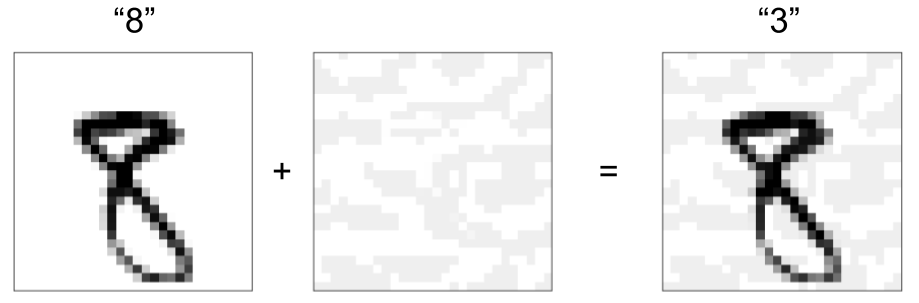
\includegraphics[width=\textwidth]{images/fgms_example.png}
        \caption{FGSM}
        \label{fgsm_example}
    \end{subfigure}
    \begin{subfigure}[b]{0.55\textwidth}
        \centering
        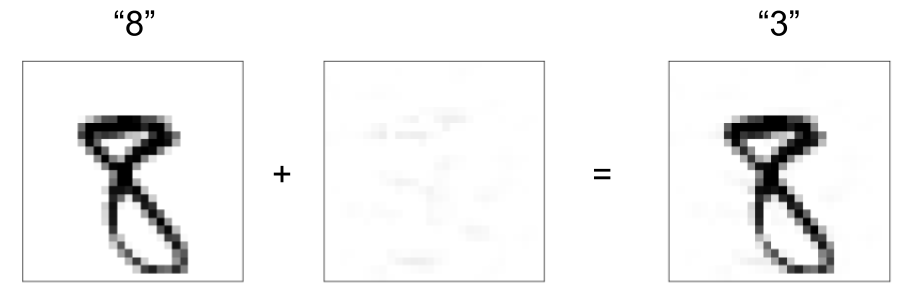
\includegraphics[width=\textwidth]{images/fgm_example.png}
        \caption{FGM}
        \label{fgm_example}
    \end{subfigure}
    \begin{subfigure}[b]{0.55\textwidth}
        \centering
        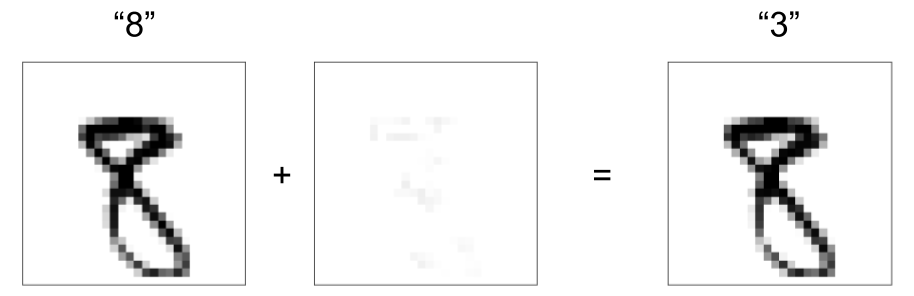
\includegraphics[width=\textwidth]{images/CW_example.png}
        \caption{CW}
        \label{CW_example}
    \end{subfigure}
    \caption{Ruido de los ataques FGSM, FGM y Carlini-Wagner sobre MNIST, con los cuales un 8 es clasificado erróneamente por la red como un 3.}
    \label{attack_examples}
\end{figure}

\subsection{Defensas}

\subsubsection{Compresión JPEG}

Las siglas JPEG vienen de "Joint Photographic Experts Group", que es el nombre del grupo que creó el estándar en 1992, el cual es una compresión con pérdida que utiliza la transformada discreta del coseno (DCT), una técnica propuesta por Nasir Ahmed en 1972, y que normalmente elimina muchos componentes de alta frecuencia, a los que la percepción humana es menos sensible \cite{das2017keeping, shaham2018defending}. Consta de los siguientes pasos:
\begin{enumerate}
    \item Conversión de la imagen de formato RGB a formato YC$_b$C$_r$, donde el canal Y representa luminancia y los canales C$_b$ y C$_r$ representan crominancia. Esto está hecho porque el sistema visual humano se basa más en el contenido espacial y la agudeza que en el color para la interpretación.
    \item Submuestreo espacial de los canales de crominancia en el espacio YC$_b$C$_r$: el ojo humano es mucho más sensible a los cambios de luminancia, y reducir la muestra de la información de crominancia no afecta mucho la percepción del ser humano de la imagen.
    \item Dividir la imagen en bloques de 8 $\times$ 8 y aplicar DCT en 2D a cada bloque. Esto se hace para cada canal por separado. Este paso produce mayor compresión de los datos de la imagen.
    \item Cuantificación de las amplitudes de frecuencia, lograda dividiendo cada término de frecuencia por una constante (diferente) y redondeándola al número entero más cercano. Como resultado, muchos componentes de alta frecuencia generalmente se establecen en cero y otros se reducen. La cantidad de compresión se rige por un parámetro de calidad especificado por el usuario, que define la reducción en la resolución. Aquí es donde el algoritmo JPEG logra la mayor parte de la compresión, a expensas de la calidad de la imagen. Este paso suprime más las frecuencias más altas, ya que estos coeficientes contribuyen menos a la percepción humana de la imagen.
    \item Compresión sin pérdidas de los datos del bloque.
\end{enumerate}

En la Figura \ref{cal_JPEG} se muestran 2 ejemplos de compresión JPEG con imágenes de MNIST (Fig. \ref{jpeg_cal_mnist}) y CIFAR-10 (Fig. \ref{jpeg_cal_cifar}), para distintos niveles de compresión, la cual aumenta como el inverso de la calidad.

\begin{figure}[h]
    \centering
    \begin{subfigure}[b]{0.48\textwidth}
        \centering
        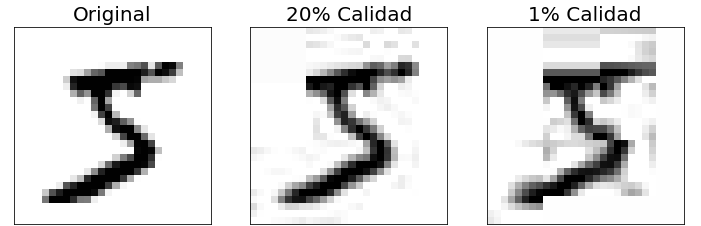
\includegraphics[width=\textwidth]{images/mnist/jpeg_qual_mnist.png}
        \caption{MNIST}
        \label{jpeg_cal_mnist}
    \end{subfigure}
    \hfill
    \begin{subfigure}[b]{0.48\textwidth}
        \centering
        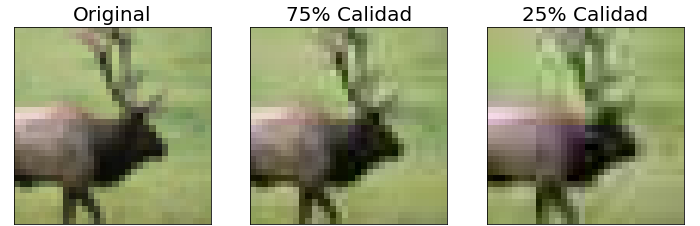
\includegraphics[width=\textwidth]{images/cifar-10/jpeg_qual_cifar.png}
        \caption{CIFAR-10}
        \label{jpeg_cal_cifar}
    \end{subfigure}
    \caption{Distintos niveles de compresión (inverso de la calidad) JPEG}
    \label{cal_JPEG}
\end{figure}